\documentclass[11pt,a4paper]{article}
%%%%%%%%%%%%%%%%%%%%%%%%%%%%%%%%%%%%%%%%%%%%%%%%%%%%%%%%
%                      PACKAGES                        %
%%%%%%%%%%%%%%%%%%%%%%%%%%%%%%%%%%%%%%%%%%%%%%%%%%%%%%%%

\usepackage[utf8]{inputenc}
\usepackage{graphicx} % Allows you to insert figures
\usepackage[export]{adjustbox}
\usepackage{booktabs}
\usepackage{amsmath} % Allows you to do equations
\usepackage{helvet}
\usepackage{hyperref}
\renewcommand{\familydefault}{\sfdefault}
\usepackage[a4paper, total={6.5in, 9.5in}]{geometry} % Formats the paper size, orientation, and margins
\linespread{1.1} % about 1.5 spacing in Word
\setlength{\parindent}{0pt} % no paragraph indents
\setlength{\parskip}{1em} % paragraphs separated by one line
\usepackage{listings}
\usepackage{enumitem}
\usepackage{xcolor}
\usepackage{hyperref}
\hypersetup{
	colorlinks=true,
	urlcolor=cyan,
	linktoc=none,
}
\usepackage{fancyhdr}
\pagestyle{fancy}
\fancyhead[L,C,R]{}
\fancyfoot[L]{Blix - AI Photo Editor}
\fancyfoot[C]{}
\fancyfoot[R]{\textbf{\thepage}}
\renewcommand{\headrulewidth}{0pt}
\renewcommand{\footrulewidth}{0.5pt}

\definecolor{codegreen}{rgb}{0,0.6,0}
\definecolor{codegray}{rgb}{0.5,0.5,0.5}
\definecolor{codepurple}{rgb}{0.58,0,0.82}
\definecolor{backcolour}{rgb}{0.95,0.95,0.92}

\lstdefinestyle{mystyle}{
backgroundcolor=\color{backcolour},
commentstyle=\color{codegreen},
keywordstyle=\color{magenta},
numberstyle=\tiny\color{codegray},
stringstyle=\color{codepurple},
basicstyle=\ttfamily\footnotesize,
breakatwhitespace=false,
breaklines=true,
keepspaces=true,
numbers=left,
numbersep=5pt,
showspaces=false,
showstringspaces=false,
showtabs=false,
tabsize=2,
}

\lstset{style=mystyle}
\def\code#1{\texttt{#1}}

%%%%%%%%%%%%%%%%%%%%%%%%%%%%%%%%%%%%%%%%%%%%%%%%%%%%%%%%
%            TITLE PAGE & TABLE OF CONTENTS            %
%%%%%%%%%%%%%%%%%%%%%%%%%%%%%%%%%%%%%%%%%%%%%%%%%%%%%%%%

\begin{document}

\begin{titlepage}
	\centering
    % \includegraphics[width=0.5\textwidth]{your_logo.png}\par\vspace{1cm}
    {\scshape\LARGE Architecture\par}
    \vspace{1.5cm}
    {\huge\bfseries Blix - AI Photo Editor\par}
    \begin{figure}[h]
        \centering % center the image
        \includegraphics[width=0.5\textwidth]{../pics/blix.png}
    \end{figure}
    \vspace{2.5cm}
    {\Large\itshape The Spanish Inquisition\par}
	\begin{tabular}{|c|c|}
		\hline
		\textbf{Name} 		& \textbf{Student Number} \\
		\hline
		Armand Krynauw		& u04868286  \\
		Jake Mileham		& u21692492  \\
		Dino Gironi			& u21630276  \\
		Karel Olwage		& u21555258  \\
		Francois Combrinck	& u21729752  \\
		\hline
	\end{tabular}
    \vfill
    {\large \today\par}
\end{titlepage}

\tableofcontents
\pagebreak

%%%%%%%%%%%%%%%%%%%%%%%%%%%%%%%%%%%%%%%%%%%%%%%%%%%%%%%%
%                MAIN DOCUMENT CONTENT                 %
%%%%%%%%%%%%%%%%%%%%%%%%%%%%%%%%%%%%%%%%%%%%%%%%%%%%%%%%

\section{Design Strategy}
The architectural design strategy for this software engineering project used two
main approaches: decomposition and design based on quality requirements.

\begin{enumerate}[label*=\arabic*.]
	\item[\textbullet] {\bf Decomposition Strategy}: The decomposition strategy
	involved breaking the system down into individual components or subsystems.
	These components were then designed and implemented independently, and their
	interactions were defined. This approach allowed for a more modular design,
	which made the system easier to understand, maintain, and extend.

	\item[\textbullet] {\bf Requirements Strategy}: The design based on quality
	requirements strategy involved identifying the key quality requirements for
	the system and then designing the system to meet those requirements. This
	approach ensured that the system would be reliable, efficient, secure, and
	usable.
\end{enumerate}

\section{Quality Requirements}
\subsection*{Performance}

Performance is pivotal to the success of this project. A bad performing system
will severly hamper the user experience and will make the systems survival unfeasible.
Due to the nature of photo editing, the system should be able to handle large
images and projects without significant lag or delay, thus it is vital that these tasks are 
not just performed well, but exceedingly well to ensure a good user experience.

{\bf Quantification}

Performance is quantified by the maximum processing time for standard photo editing operations.
The Throughput and resource utilization of the system must also be investigated for the purposes
of the Blix system.

The maximum processing time of the system is measured by the time it takes to perform a standard photo editing operation
immediately after the user has requested the operation. The standard photo editing operations are defined as the following:
\begin{enumerate}
    \item Adjusting the white balance
    \item Adjusting the hue
    \item Adjusting the exposure
    \item Adjusting the saturation
    \item Rotating the image
    \item Cropping the image
    \item Applying a filter to the image
\end{enumerate}

The throughput of the system is measured by the number of standard photo editing operations that can be performed in a given time period.

The resource utilization of the system is measured by the amount of memory and CPU usage of the system during runtime.


{\bf Targets}

The target maximum processing time of the system is 1 second for a standard photo editing operations

The target throughput of the system is 5 standard photo editing operations per second.

The target resource
utilization of the system is :
\begin{enumerate}
    \item Less than 100 MB of memory and 10\% CPU usage for the minor photo editing operations
    \item 500MB of memory and 50\% CPU usage for the standard photo editing operations. 
    \item 1GB of memory and less than 90\% CPU usage for the major photo editing operations.
\end{enumerate}

\subsection*{Reliability}

The reliability of the system is dependent on the ability of the system to prevent and recover from failures.
The system should be able to prevent failures by ensuring that the system is always in a consistent state.
The system should be able to recover from failures by ensuring that the system can be restored to a consistent state, such that 
the user does not lose any work.

{\bf Quantification}

The reliability of the system is quantified by the the mean time between failures (MTBF) and the mean time to recovery (MTTR).
Another metric that will be used to quantify the reliability of the system is the number of critical failures per month.

The mean time between failures is measured by the number of operations performed by the system before a failure occurs. This number
is then divided by the number of failures that occured during the time period. 


The mean time to recovery is measured by the number of operations required to restore the system to a consistent state after a failure has occured.

The number of critical failures per month is measured by the number of failures that occured during the month that resulted in the loss of data or the loss of the ability to perform photo editing operations.

{\bf Targets}

The target mean time between failures is 100 operations.

The target mean time to recovery is 10 operations.

The target number of critical failures per month is 0.



\subsection*{Usability} 

The usability of the system is dependent on the ability of the system to be easily used by the user. It is important that the system is easy to use and that the 
user is able to perform the desired tasks with ease and with clearly defined steps. The system caters for all users, from novice to expert, thus it is important to note that not all users
will be familiar with the system and features, thus the system must provide alternatives for these users

{\bf Quantification}

To properly quantify Usability, user satisfaction cannot be neglected. Additionally the learning curve of the system must be investigated to ensure that the system is easy to use.
Finally the number of user requests completed per month must be investigated to ensure that the system is able to appeal to the users.

User satisfaction is measured by the number of users that are satisfied with the system. This number is then divided by the total number of users that used the system during the time period.

The learning curve of the system is measured by the number of operations required to perform a standard photo editing operation. This number is then divided by the number of operations required to perform the same operation on a standard photo editing software.

The number of user requests completed per month is measured by the number of requests that were fulfilled during the month. This number is then divided by the total number of requests that were made by users during the month.

{\bf Targets}

The target user satisfaction is 90\%.

The target learning curve is 1.5 times the number of operations required to perform the same operation on a standard photo editing software. 

The target number of user requests completed per month is 60\%.

\subsection*{Security} 

Security is an extension of the reliability of the system. It is important that the system is able to prevent and recover from security breaches to protect user.
At the same time, extensive security hampers the usability of the system, thus it is important to find a balance between security and usability to provide the best 

{\bf Quantification} 

Security will be conceptually quantified by the integrity , confidentiality and availability of the system.

The integrity of the system is measured by the systems transparency regarding the users limitations the policies of the system.

The confidentiality of the system is measured by how secure the user's personal details are from other users. This is measured by the amount of security measures that are in place and the number of violations that have occured.

The availability of the system is measured by the amount of systems that the users are provided access to to customize and modify.

{\bf Goals}

The integrity of the system must be well defined and transparent to the user.

The confidentiality of the system must be extremely well guarded and the number of violations must be 0.

The system must have a high availability such that the users must be able to customize and modify the system to their liking.

\subsection*{Compatibility} 

Compatibility is an extremely important quality requirement for the system. The
system must be able to run on a variety of platforms and must be able to support
a variety of image formats. Due to the nature of the system, extensive
compatibility is required to ensure that the system is able to appeal to a wide
range of users.

{\bf Quantification}

Compatibility is quantified by the number of platforms that the system is able
to run on and the number of image formats that the system is able to support.

The number of platforms that the system is able to run on is measured by the
number of platforms that the system is able to run on, with a specific focus on
the most popular platforms.

The number of image formats that the system is able to support is measured by
the number of image formats that the system is able to support, with a specific
focus on the most popular image formats.

{\bf Goals}

The system should be compatible with all the most well-known platforms : 
\begin{enumerate}
    \item Windows
    \item Linux
    \item Mac OS
\end{enumerate}

The system should be compatible with all the most well-known image file formats : 
\begin{enumerate}
    \item JPEG
    \item PNG
\end{enumerate}


\pagebreak

\section{Architectural Design \& Patterns}
Four main architectural patterns where identified to decompose the base system
into components and subsystems.

\begin{figure}[ht]
	\centering
	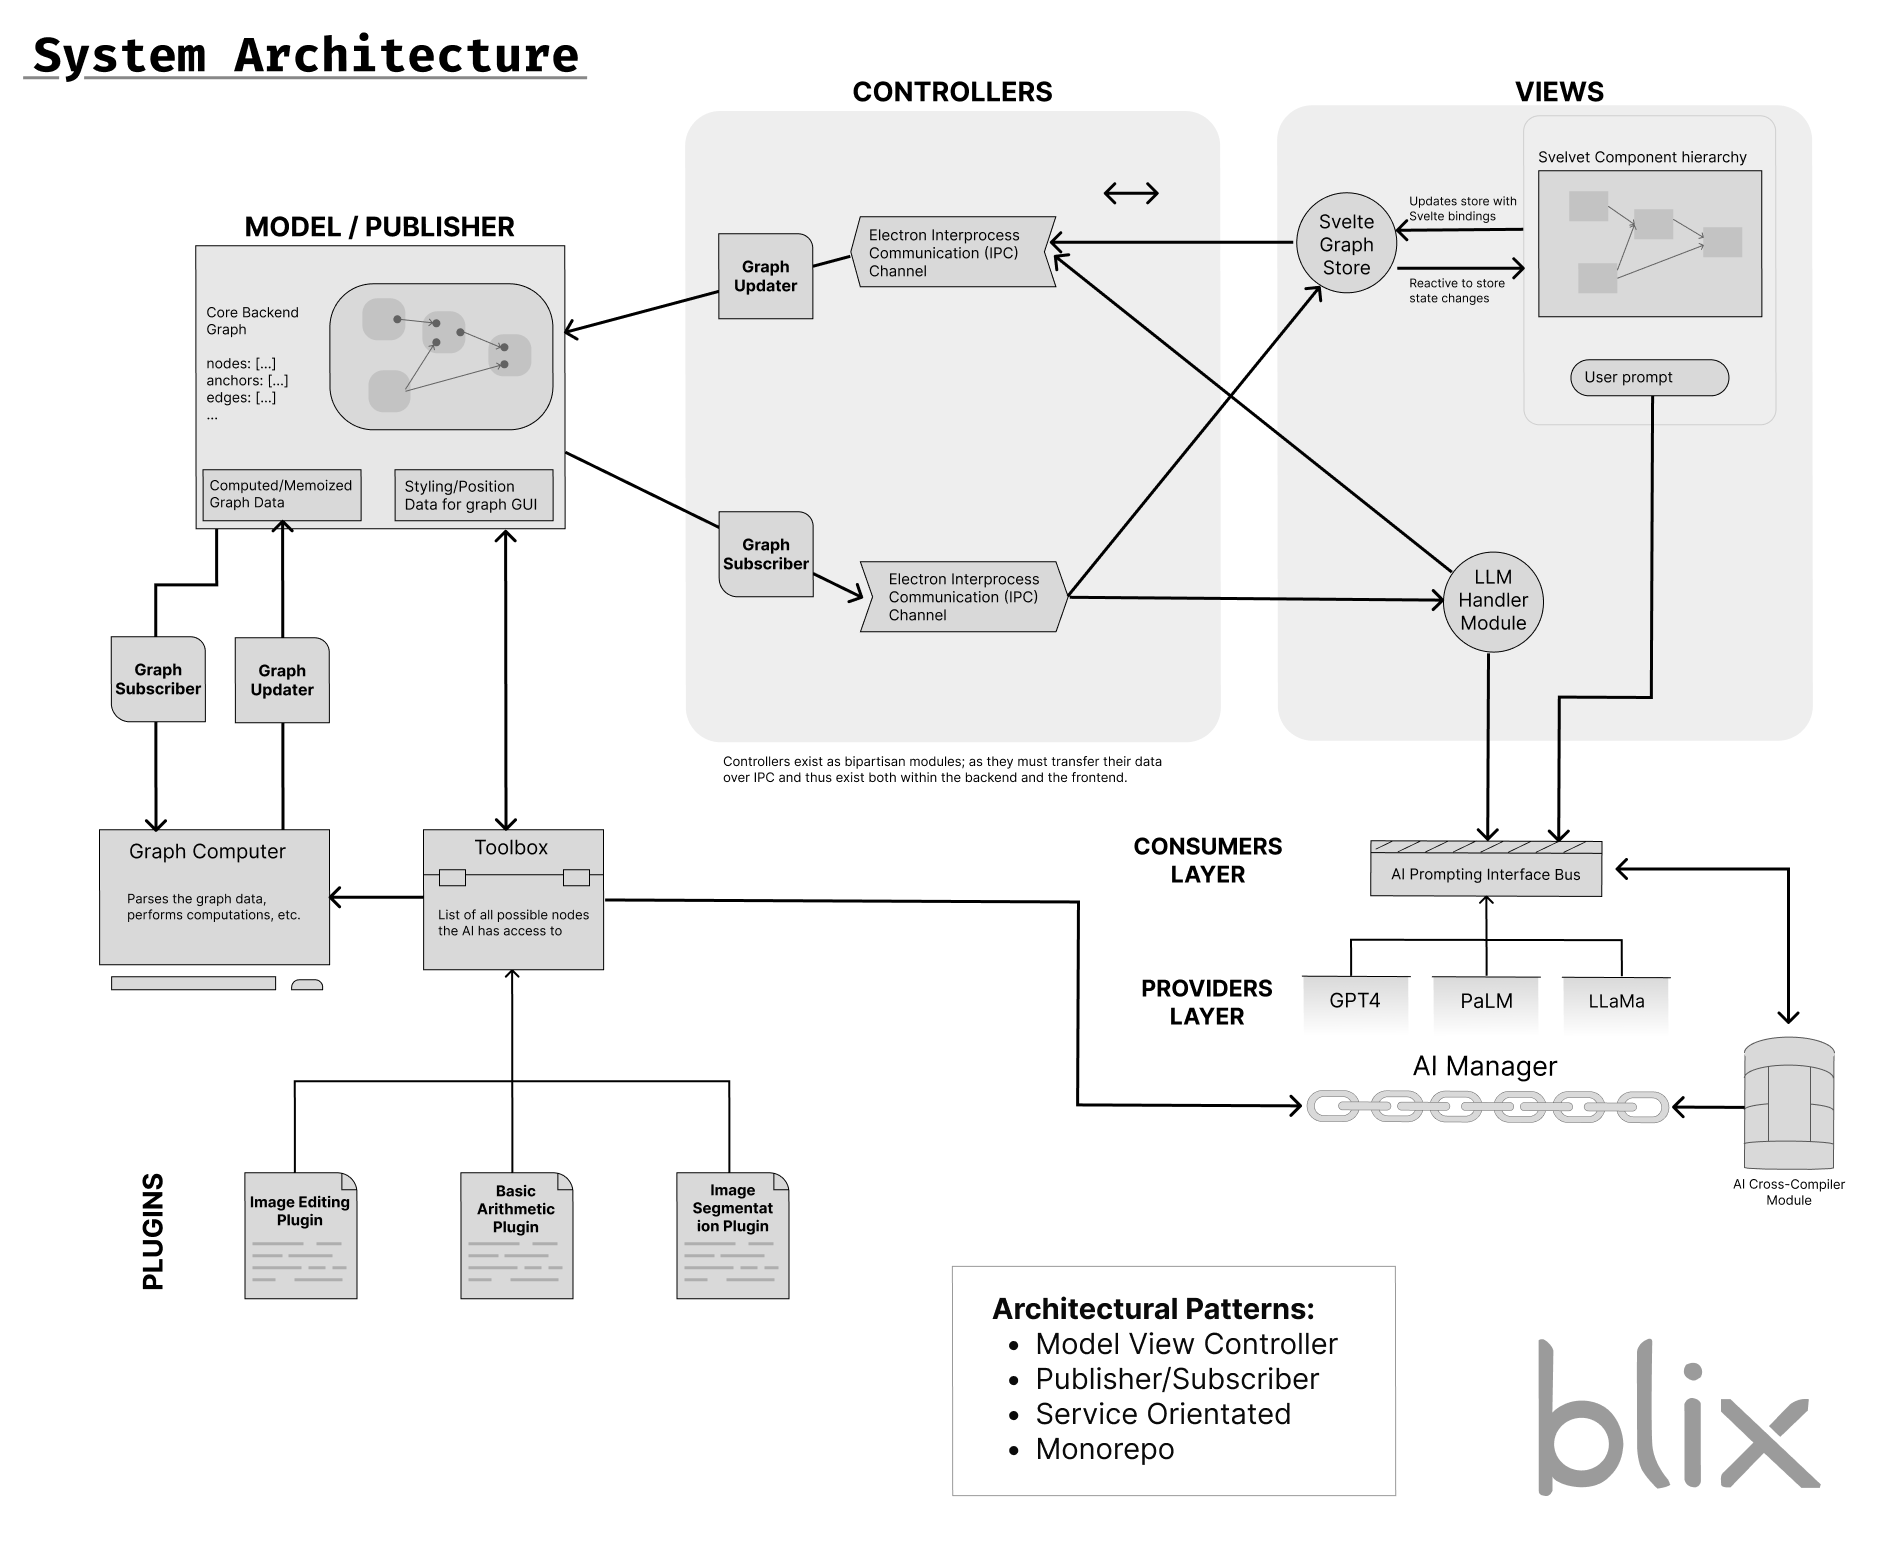
\includegraphics[width=1\textwidth,height=\textheight,keepaspectratio,rotate=0,origin=c]{../diagramPng/System_Architecture1.png}
\end{figure}

\subsection{Model-View-Controller (MVC)}
The MVC pattern was chosen in order to create clear distinction between the user
interface, business logic and system data. This trinity-based setup enables
separation of concerns and allows for the system to be easily extended and
maintained. Each of the three components play their parts as follows:
\begin{enumerate}[label*=\arabic*.]
	\item[\textbullet] {\bf Model}: The 'model' in our system is the core
	backend graph running on the Node.js server within the Electron application.
	This represents the core state of the system, and is the central source of
	truth for all other views in the system. In a sense, it acts as a central
	database which all other 'services' utilize.
	\item[\textbullet] {\bf Views}: Our system consists of multiple views which
	all derive representations from the core graph {\it model}. Some examples of
	views in the system include the frontend {\it Svelvet} graph which the user
	interacts with, as well as the text-based (e.g. JSON) model which is passed
	to the LLM AI assistant. When changes take place within the core graph,
	these views are automatically updated to reflect them.
	\item[\textbullet] {\bf Controllers}: These are the 'middle-men' between
	each view, and the core graph. As our system is an Electron application, the
	frontend views must be able to communicate with the core graph over
	Electron's IPC ({\it Interprocess Communication}) protocol.

	When changes to local view state take place (e.g. If the user were to add a
	new node to the frontend graph), the controllers are responsible for
	instructing the core backend graph that these changes have taken place. Then
	after the core graph has applied these changes in a manner that is
	consistent (forms a valid directed compute graph), all subscriber views are
	notified of the changes and are updated accordingly.
\end{enumerate}


\subsection{Publish-Subscribe}
Our implementation layers the Publish-Subscribe architectural pattern on top of
the MVC pattern to endow the system with multiple-reactivity. The PubSub
architecture allows one central source of information to be propagated to a
multitude of subscribers, in our case the core graph and each of its views
respectively. PubSub is a highly effective pattern as it abstracts the notion of
state propagation into a composable set of participant modules which can be
easily added/removed from the system. This helps us future-proof the application
and allows for scalability as the system grows.

As an example, let's say down the line we wanted to add a command line utility
to compute a given graph without needing the user interface to be loaded; In
such a situation we could easily disable the UI graph subscriber, and add
alongside a 'command line utility' subscriber, which still communicates with the
core graph, but does so entirely through the standard input/output streams of
the command line.

Thus by using this architecture we have effectively made core parts of the
system 'hot-swappable'.

\subsection{Service-Oriented}
The Service-Oriented architectural pattern exists within an essential aspect of our system, the AI LLM assistant.
This pattern enables modularity, flexibility, and extensibility by defining the system's components as a collection of distinct services.
Here we treat each LLM model as a separate service, which can be added, removed, or swapped out with another model.

Models that may be supported as 'services' include GPT-3, GPT-4, PaLM, etc.
Each of these models can subscribe to the core graph and make updates to it.
Moreover, by leveraging the power of LangChain using a custom pre-trained vector database of graph {\it word2vec} embeddings,
the Service-Oriented architecture helps us to create a comprehensive and efficient system for managing these models and enhancing their capabilities with domain-specific knowledge.

This allows for seamless exchanging of information among the services, as well as smooth updating and enhancement of the system when new AI models become available or when updates to existing models are released.
Consequently, the Service-Oriented architecture maximizes the potential of our AI-driven system by promoting modularity, interoperability, and the rapid development of new features and capabilities.


% \subsection{Client-Server}
% The Large Language Model AI assistant is a significant part of the system which
% we are building, and at the time of writing all major LLMs (which provide the
% sufficient level of intelligence that we are looking for) are hosted on the
% cloud. As our app is hosted natively on this users machine, this means we must
% also enable remote communication to the respective LLM API's.

% From this perspective, the Blix application exists as a client to the LLM API
% server, and must be able to perform remote HTTP requests as such. Google has
% recently announced the release of their PaLM models as open source, however, and
% so we are currently investigating the possibility of hosting the LLM locally on
% the users machine. In such a situation the client-server architecture would
% still apply, except that the server 'LLM API' would be hosted locally on the
% users machine, and all communication would be done over the loopback interface.


\section{Constraints}

No special constraints or limitations have been identified or explicitly
communicated by the client.

\section{Technology Choices}

\subsection{Svelte}
Svelte is an open-source JavaScript framework for building user interfaces. It
is designed to be highly efficient and focused on delivering optimal performance
by shifting the work from the runtime to the build process. One of the key
visions of Blix is to provide a fast and responsive user interface with
lightning fast reactivity. Additionally due to the large scope of the project,
it is important to ensure that the system is as lightweight as possible. Svelte
is the perfect choice for this as it compiles the application into highly
performant JavaScript, instead of simulating a virtual DOM for performing
reactive page updates.

\textbf{Pros:}
\begin{enumerate}[label*=\arabic*.]
	\item[\textbullet] Fast and responsive user interface with lightning fast
	reactivity. 
	\item[\textbullet] Svelte is a highly scalable framework that allows for the
	creation of large scale applications.
	\item[\textbullet] Reusability of components shortens development time.
\end{enumerate}


\textbf{Cons:}
\begin{enumerate}[label*=\arabic*.]
	\item[\textbullet] Svelte is a relatively new framework and as such has a
	smaller community than other frameworks such as React and Vue.
	\item[\textbullet] Svelte has a smaller ecosystem than other frameworks such
	as React and Vue.
	\item[\textbullet] Svelte is lacking in stability as it is still a
	relatively new framework.
\end{enumerate}

\subsection{Tailwind CSS}
Tailwind CSS is an utility-first CSS framework that provides a set of
pre-designed, low-level utility classes. Tailwind CSS focuses on providing a
comprehensive set of utility classes that you can combine to build custom user
interfaces. Tailwind CSS is the perfect choice for Blix as it allows for the
creation of a custom user interface that is unique to Blix. Additionally,
Tailwind CSS is highly scalable and allows for the creation of large scale
applications.

\textbf{Pros:}
\begin{enumerate}[label*=\arabic*.]
	\item[\textbullet] Tailwind CSS is a scalable framework that allows for the
	creation of large scale applications.
	\item[\textbullet] Tailwind CSS is a customizable framework that allows for
	the creation of a custom user interface that is unique to Blix.
	\item[\textbullet] Tailwind CSS is a responsive framework that allows for
	the creation of a responsive user interface.
\end{enumerate}

\textbf{Cons:}
\begin{enumerate}[label*=\arabic*.]
	\item[\textbullet] The class names can make the HTML markup harder to read
	and maintain, especially for larger projects.
	\item[\textbullet] Tailwind CSS generates a large CSS file due to the
	extensive collection of utility classes. 
	\item[\textbullet] The class names can make the markup harder to read and
	maintain, especially for larger projects.
\end{enumerate}

\subsection{Electron}

Electron allows developers to build cross-platform desktop applications using
web technologies such as HTML, CSS, and JavaScript. Electron allows developers
to locally host a web application within a desktop application. This allows for
the creation of a desktop application that is highly scalable and can be easily
ported to other platforms.
\textbf{Pros:}

\begin{enumerate}[label*=\arabic*.]
	\item[\textbullet] Highly scalable framework that allows for the creation of
	large scale applications.
	\item[\textbullet] Electron provides a comprehensive set of APIs that allows
	for the creation of a desktop application that is unique to Blix.
	\item[\textbullet] Allows code reuse as the same codebase can be used to
	create a desktop application and a web application.
	\item[\textbullet] Leverages the power of Node.js modules to provide 
\end{enumerate}
\pagebreak
\textbf{Cons:}

\begin{enumerate}[label*=\arabic*.]
	\item[\textbullet] Electron generates a large executable file due to the
	extensive collection of APIs.
	\item[\textbullet] High memory usage due to the extensive collection of
	APIs.
	\item[\textbullet] Dependent on chromium browser updates.
\end{enumerate}


\subsection{Firebase}

Firebase is a mobile and web application development platform developed by
Firebase, Inc. in 2011, then acquired by Google in 2014. Firebase provides a
comprehensive set of APIs that allows developers to build, manage, and deploy
applications. Firebase is the perfect choice for Blix as it provides a
comprehensive set of APIs that allows for the creation of a highly scalable
application.

\textbf{Pros:}
\begin{enumerate}[label*=\arabic*.]
	\item[\textbullet] Real time database that allows for the creation of a
	highly scalable application.
	\item[\textbullet] Cloud storage that allows for efficient data storage and
	retrieval.
	\item[\textbullet] Quick and easy authentication that allows for the
	creation of a secure application.
\end{enumerate}

\textbf{Cons:}
\begin{enumerate}[label*=\arabic*.]
	\item[\textbullet] Lack of flexibility as Firebase is a closed source
	platform.
	\item[\textbullet] Limited server side logic as Firebase is a closed source
	platform.
	\item[\textbullet] Scalability and latency considerations is an external
	service.
\end{enumerate}


\subsection{LangChain}

Langchain is a new framework built around llm that allows developers to build
applications that capitalize on the knowledge base and computational power of 
llm's such as gpt-3 by provided the llm's with specialized knowledge on the 
applications domain. Langchain is usefull for Blix as it allows for the manipulation
of the graph and photos using natural language and llms. 

\textbf{Pros:}
\begin{enumerate}[label*=\arabic*.]
	\item[\textbullet] Local storage of context and knowledge base.
	\item[\textbullet] Chaining of llm's to exploit different llm's strengths.
	\item[\textbullet] Allows for the creation of a highly scalable application.
	\item[\textbullet] Flexibility as Langchain is an open source platform.
\end{enumerate}

\textbf{Cons:}
\begin{enumerate}[label*=\arabic*.]
	\item[\textbullet] Lack of solid documentation as Langchain is a new framework.
	\item[\textbullet] Generally requires more requests to llm's to achieve the desired result.
	\item[\textbullet] Lack of integrations for a typescript environment.
\end{enumerate}

\subsection{PineCone}

PineCone is a vector database which allows developers to build, manage, and search
embeddings using optimized storage and querying abilities that better suit the complexities
and size of the data from embeddings then traditional databases. PineCone is used in Blix
to store and query the embeddings of our knowledge base to provide short and efficient contexts
to llm's.

\textbf{Pros:}
\begin{enumerate}[label*=\arabic*.]
	\item[\textbullet] Enables easy integration with AI related technologies.
	\item[\textbullet] Can store metadata associated with each entry for finer grained queries.
	\item[\textbullet] High performance and low latency.
\end{enumerate}

\textbf{Cons:}
\begin{enumerate}[label*=\arabic*.]
	\item[\textbullet] Relies heavily on the quality of input data.
	\item[\textbullet] Requires a large amount of data to be effective.
	\item[\textbullet] High complexity indexing.
\end{enumerate}

\subsection{typescript}

typescript is a superset of javascript that adds static typing to javascript. typescript
is used in Blix to provide a more robust codebase and to minimize the number of runtime errors
that can occur. typescript is a versatile language that allows for the creation of a 
stable application.

\textbf{Pros:}
\begin{enumerate}[label*=\arabic*.]
	\item[\textbullet] Any valid javascript code is valid typescript code.
	\item[\textbullet] Type system allows for the minimization of runtime errors.
	\item[\textbullet] Better maintainability and documentation of code as typescript is a strongly typed language.
\end{enumerate}

\textbf{Cons:}
\begin{enumerate}[label*=\arabic*.]
	\item[\textbullet] Additional developement overhead
	\item[\textbullet] More limited ecosystem
\end{enumerate}

\subsection{Nodejs}

Nodejs is an open source, cross-platform, back-end javascript runtime environment that
executes javascript code outside of a web browser. Nodejs is used in Blix to provide a
stable and high performance back-end for our application.

\textbf{Pros:}
\begin{enumerate}[label*=\arabic*.]
	\item[\textbullet] Everything can be done in typescript
	\item[\textbullet] Vast ecosystem of libraries and frameworks
	\item[\textbullet] High performance and low latency
\end{enumerate}

\textbf{Cons:}
\begin{enumerate}[label*=\arabic*.]
	\item[\textbullet] Single threaded event loop
	\item[\textbullet] Relatively high memory usage
\end{enumerate}

\subsection{Python}

Python is an interpreted language that provides a large standard library and a vast ecosystem
of libraries and frameworks. Python is used in Blix to provide a stable and high performance
environment for our AI assistant such that langchain can be used to its full potential.

\textbf{Pros:}
\begin{enumerate}[label*=\arabic*.]
    \item [\textbullet] Large standard library
	\item [\textbullet] versatile and flexible
	\item[\textbullet] Great integration with Langchain
\end{enumerate}

\textbf{Cons:}
\begin{enumerate}[label*=\arabic*.]
	\item[\textbullet] Expensive	
	\item[\textbullet] Volatile type checking
	\item[\textbullet] Performance
	\item[\textbullet] Dependency management is complicated for blix
\end{enumerate}

\subsection{Jest}

Jest is a javascript testing framework that is used in Blix to provide a stable and
reliable codebase. Jest is used to test the functionality of our application and to
ensure that our application is working as intended. We picked jest as our testing
framework as it is the most popular testing framework for javascript and it is
recommended by the creators of typescript.

Here are more of the considerations that we took into account when choosing a testing
framework:

\textbf{Pros:}
\begin{enumerate}[label*=\arabic*.]
    \item [\textbullet] Fast and efficient
	\item [\textbullet] Great documentation
	\item [\textbullet] Built-in code coverage
\end{enumerate}

\textbf{Cons:}
\begin{enumerate}[label*=\arabic*.]
	\item[\textbullet] Size and Complexity	
	\item[\textbullet] Configuration Overhead
\end{enumerate}

\subsection{AI Models}

Blix supports multiple language models, each with their own strengths and weaknesses.
The language models are used in Blix to provide a more natural and human like experience
while also allowing the user to fine tune their experience to their liking.

Below is a list of the language models that Blix supports:

\subsection{GPT-3.5 Turbo}

\textbf{Pros:}
\begin{enumerate}[label*=\arabic*.]
    \item [\textbullet] Great performance and reasoning
	\item [\textbullet] versatile and flexible
	\item[\textbullet] Well known and documented
\end{enumerate}

\textbf{Cons:}
\begin{enumerate}[label*=\arabic*.]
	\item[\textbullet] Expensive	
	\item[\textbullet] Limited to textual input and output
\end{enumerate}

\end{document}